\documentclass[twoside,11pt]{article}
\usepackage{jmlr2e}
\usepackage{graphicx}
\graphicspath{ {./images/} }
\usepackage{enumitem}
\newlist{mylistenv}{enumerate}{3}
\newenvironment{mylist}[1]{%
	\setlist[mylistenv]{label=#1\arabic{mylistenvi}.,ref=#1\arabic{mylistenvi}}%
	\setlist[mylistenv,2]{label=#1\arabic{mylistenvi}.\arabic{mylistenvii}.,ref=#1\arabic{mylistenvi}.\arabic{mylistenvii}}%
	\setlist[mylistenv,3]{label=#1\arabic{mylistenvi}.\arabic{mylistenvii}.\arabic{mylistenviii}.,ref=#1\arabic{mylistenvi}.\arabic{mylistenvii}.\arabic{mylistenviii}}%
	\renewenvironment{mylist}{\begin{mylistenv}}{\end{mylistenv}}
	\begin{mylistenv}%
	}{%
	\end{mylistenv}%
}
\newcommand\tab[1][1cm]{\hspace*{#1}}

% Definitions of handy macros can go here

\newcommand{\dataset}{{\cal D}}
\newcommand{\fracpartial}[2]{\frac{\partial #1}{\partial  #2}}


\firstpageno{1}

\begin{document}

\title{Project 4: Networks for Classification and Regression}

\author{\name Sarah Wilson 
	   \email swi1s117@jhu.edu \\
	   \phone 303-921-7225 \\
       \addr Engineering Professionals Computer Science\\
       Johns Hopkins University\\
       Baltimore, MD 21218, USA} 

\maketitle


\section{Introduction}
\hspace*{10mm} Neural Networks are collection of algorithms that are taught the underlying patterns in a data set through a process of supervised learning. Neural Networks operate using a process that is similar to the human brain, they contain simple processing nodes, called neurons that are connected in layers. These layers contain weights that determine an output based on a given input. The basis of an understanding of Neural Networks actually starts with Linear Regression.\\ 
\hspace*{10mm} Linear Regression is a supervised Machine Learning algorithm that can be applied to Regression problems. Linear Regression assumes there is some sort of linear relationship between the input data and the output value that can be represented by a line or plane of best fit between the inputs and the output. Linear Regression is meant for continuous outputs, when Classification tasks are required (tasks that have outputs with class labels), then the concepts of linear regression can be applied, but instead the Sigmoid function is used, hence the name Logistic Regression. The sigmoid function is able to take classifiers that are not numeric and map them to values between 0 and 1. Linear and Logistic regression are the basic concepts that build the foundation for Neural Networks. Neural Networks can be thought of as a series of Logisitc regression tasks that happen across many layers and nodes. Neural Networks can also be augmented through the use of developing an Auto Encoder. The Auto Encoders are trained such that an output pattern to a network always matches the input pattern. The Auto Encoder process can be thought of a method to fine tune the weights feeding the prediction output from a Neural Network.\\
\hspace*{5mm} The problem statement presented in this paper is to understand an implement three major categories of networks; Linear, Feed-Forward Back Propagation and  Feed-Forward Back Propagation with an Auto Encoder. For the Linear Network: a Linear Regression will be applied to Regression problems while a Logistic Regression will be applied to the Classification Problems.\\
\hspace*{5mm} The hypothesis of this report is that the  Feed-Forward Network with an Auto Encoder will perform better than the Feed-Forward Back Propagation and Linear regression approaches on both the Classification and Regression problems. The reason for this hypothesis is that the Auto Encoder builds upon the Linear Regression and basic Neural Regression. Both Linear Regression and Neural Networks rely on updating weight based on the error between the predicted output and the actual output of a training set. The Auto Encoder improves upon this process by trying to learn and mimic the input pattern of the data and apply that to the output or predicted value. This extra encoding and decoding steps, serve to fine tune the weights feeding the neural network. The hypothesis is based around the concept that fine tuned weights should out preform coarsely tuned weights in making predictions based on new input data to the network. The results from experiments ran on the provided data sets will be discussed and presented against the outlined hypothesis.\\
\hspace*{5mm} Section 1 has provided the introduction, problem statement and hypothesis in regards to three major learning algorithms that will be explored. Section 2 will provide an in-depth explanation of the algorithms. Section 3 will present the results obtained by the different algorithms. Section 4 will discuss the results that were obtained and compare them to the hypothesis that was outlined in the introduction. This report will conclude in Section 5 with a discussion of lessons learned and areas of possible future work.\\


\section{Algorithms and Experimental Methods}
\hspace*{10mm} \textbf{Linear and Logistic Regression}\\
\hspace*{10mm} Regression is an a problem solving approach in Machine Learning that models a target predictor based on independent variables or values.  Linear Regression and Logistic Regression both are discriminant-based approaches that do not care about estimating the densities inside a particular class region, instead the discriminant-based approach aims to estimate the boundaries between the class regression. The output of Linear and Logistic regression models is a weighted sum of the input attributes or features. The magnitude of the weight applied against each feature, shows the importance of that feature towards the overall prediction. The weights are learned by the model during training. Linear Regression is used on Regression problems because the data that is being predicted is continuous. This Linear model will not work for Classification problems, as the output of the linear model would be a real value, when in Classification a class label is desired. Logistic Regression is used for Classification problems, as it maps the output of the weight sum presented in Linear Regression and maps it to a non-linear function that ensures the outputs are between 0 and 1. The function used to achieve this is the Sigmoid or Logistic function.\\
\hspace*{10mm} The objective of training in both Linear and Logistic Regression is to determine the weights that will be used in the final model. The weight coefficients can be determined using the process of Gradient Descent. The general procedure for applying Gradient Descent is to first calculate the prediction based on the current weight coefficients and then calculate new coefficients based off the error in the prediction. This process is repeated until the coefficients are deemed accurate enough. The weight convergence process used in this paper to determine if the prediction is accurate enough will be to a set number of iterations. After the set number of iterations through the weight update process, the weights will be deemed good enough. At this point the model can be considered trained and will be evaluated for performance on the test data set.
\newpage

\textbf{Linear and Logistic Regression Algorithm}\newline
For each Feature (\textit{j}) in the Domain(\textit{d}) of the Data Set:\\
\tab Set $W_j$ to a random value between -0.01 and 0.01\\
For Each Step in the Number of Iterations for Convergence:\\
\tab For each Feature (\textit{j}) in the Domain(\textit{d}) of the Data Set:\\
\tab \tab $\Delta W_j$ = 0\\
\tab For each observation (\textit{t}) in the Data Set:\\
\tab \tab Set the Temp Prediction (\textit{o}) to 0.\\
\tab \tab \tab For each Feature (\textit{j}) in the Domain(\textit{d}) of the Data Set:\\
\tab \tab \tab \tab  (\textit{o}) =  (\textit{o}) + $W_j * X_j$\\
\tab \tab \tab If the problem is Regression:\\
\tab \tab \tab \tab Set the Model Prediction (\textit{y}) to the Temp Prediction Value (\textit{o})\\
\tab \tab \tab If the problem is Classification:\\
\tab \tab \tab \tab Set the Model Prediction (\textit{y}) to the Sigmoid(\textit{o})\\
\tab \tab \tab For each Feature (\textit{j}) in the Domain(\textit{d}) of the Data Set:\\
\tab \tab \tab \tab $\Delta W_j$ = $\Delta W_j + (r - y)X_j$\\
\tab For each Feature (\textit{j}) in the Domain(\textit{d}) of the Data Set:\\
\tab \tab $W_j$ = $W_j + \eta \Delta W_j $\\

Where $\eta$ is the learning rate.\\
Note that the algorithm shown above is can be used for both Regression and Classification. However, for Classification only the two class problem is shown. This algorithm can be expanded to include a multiple class Classification problem.\newline  

\hspace*{10mm} \textbf{Linear Neural Networks}\\
\hspace*{10mm} With a basic understanding of the Linear and Logisitc regression algorithms, these processing techniques can be expanded to build a Neural Network. For the purposes of this paper the Linear Neural Network will be built with a Input Layer, Two Hidden Layers and the Final Output Layer. The structure of a Neural Network is something that can be tuned and tweaked to provide different results, that fell outside the scope of work for this paper, however provides an area of future work. The structure used for the Neural Network in this paper, has the number of nodes in each layer being equal to the number of features in the data set. In other words, the number of nodes in the hidden layers is equal to the domain of the data set. The neurons in each of the layers are connected by edges and those edges are tied to weight values. The algorithm explored in this paper is Back Propagation. The general idea behind Back Propagation is to model a pattern or model in the data set by modifying the weight of the internal network structure. This network is trained using supervised learning, where the error between the predicted value and the actual output value of an observation, is used to back propagate and update the weights of the edges inside the Network.\\
\hspace*{10mm} An observation is fed forward through the network, using an initial set of weights. As each feature in the input data set passes through a Neuron the Neuron is activated, as in the input feature times the weight connecting the feature to that neuron is calculated and then passed through the Sigmoid function. The Sigmoid function is used for the activation function in the neurons for both Classification and Regression problems.\\
\hspace*{10mm} The difference between the Classification and Regression problems comes about in the output layer of the network. For a two class Classification problem, there is only one output node and if the output node is between 0 and 0.5, then the data will be classified as class A. If the output node is above 0.5 to 1, then the data will be classified as class B. If it is a multiple class classification (greater than 2 classes), then there are as many output nodes as there are classes and the soft max function is used to chose the node with the largest value, the data will then be classified according to the class output node that contains the highest value.  In regression, there is also only one output node, but the value stored in that output node is the continuous value predicted by the data.\\ 
\hspace*{10mm} In order to train the weights inside the network, a technique is used called back propagation. An observation is fed forward, and then the error between the predicted and actual output is propagated back through the network, so that each weight connecting each node is adjusted for the error it contributed to the final output. This is done by using Gradient Descent and feeding back the derivative of the Sigmoid function to each Neuron. The weights are trained using this process and presented in this paper as a number of iterations until the weights have converged.\\

\textbf{Linear Neural Networks Algorithm}\newline
Build Network with the Desired Number of Hidden Layers and Nodes in Each Layer.\\
For each Edge connecting a node to another node in the network, set the Weight to a random value between (-0.01 and 0.01) \\
For Each Step in the Number of Iterations for Convergence:\\
\tab For each observation (\textit{t}) in the Train Data Set:\\
\tab \tab \textbf{Feed Forward}\\
\tab \tab \tab For Each Layer in the Network:\\
\tab \tab \tab \tab If the input layer use the observation as the data into the Neuron.\\
\tab \tab \tab \tab If any other layer use last layers output as the data the Neuron.\\
\tab \tab \tab \tab  For Neuron in the Layer:\\
\tab \tab \tab \tab \tab Calculate the Activation At the Neuron..\\
\tab \tab \tab \tab \tab Store that Neuron Output in the Neuron.\\
\tab \tab \textbf{Back Propagate} \\
\tab \tab \tab Reverse the Order of the Network (so the the output layer is first).\\
\tab \tab \tab For Each Layer in the Reversed Network:\\
\tab \tab \tab \tab If output layer:\\
\tab \tab \tab \tab \tab Calculate the error between the neuron output and the actual\\ 
\tab \tab \tab \tab \tab data set predictor. $(r-y)$\\
\tab \tab \tab \tab Calculate the derivative of the Sigmoid function, using the Neurons\\
\tab \tab \tab \tab current output.\\
\tab \tab \tab \tab Update the Neurons Updated Weight  = $error - sigmoid derivative$\\
\tab \tab \tab \tab If any other Layer:\\
\tab \tab \tab \tab \tab For Node in Layer:\\
\tab \tab \tab \tab \tab \tab Update the Neurons Weight\\
\tab \tab \tab \tab \tab \tab Updated Weight = Updated Weight * Current Weight\\
\tab \tab Re-Reverse the Network to return the original network with new\\ 
\tab \tab updated weights.\\
\tab Once Weights have Converged:\\
\tab For each observation (\textit{t}) in the Test Data Set:\\
\tab \tab Run the Steps listed under \textbf{Feed Forward}\\
\tab Return a list of predictions for every observation in the Test Data Set.\\

\hspace*{10mm} \textbf{Auto Encoded Linear Neural Networks}\\
\hspace*{10mm} An Auto Encoded Linear NN is a variation of the Linear NN algorithm described previously. The intent of the Auto Encoded is to act as a de-nosing technique for the training of weights for the Linear Neural Network. The Auto Encoded Network is built with an input layer that has as many nodes as the input data set has features. There is one hidden layer and one output layer, both with the same number as nodes as the input layer. This Network has its weights trained using the same Back Propagation method discussed in the previously. Once the training has completed the Auto Encoded Hidden Layer weights are used to seed the first hidden layer weights of the Linear NN (instead of seeding them to random values between -0.1 and 0.1). In essence the Auto Encoded acts as a fine tuner of the weights using the data sets prior to running the full Linear NN. \\

\textbf{AutoEncoded Linear Neural Networks Algorithm}\newline
\textbf{Start Process for the Auto Encoded Neural Network}\\
Build Network with the One Hidden Layer, with a number of nodes equal to the domain of the input.\\
For each Edge connecting a node to another node in the network, set the Weight to a random value between (-0.01 and 0.01) \\
For Each Step in the Number of Iterations for Convergence:\\
\tab For each observation (\textit{t}) in the Train Data Set:\\
\tab \tab \textbf{Feed Forward}\\
\tab \tab \tab For Each Layer in the Network:\\
\tab \tab \tab \tab If the input layer use the observation as the data into the Neuron.\\
\tab \tab \tab \tab If any other layer use last layers output as the data the Neuron.\\
\tab \tab \tab \tab  For Neuron in the Layer:\\
\tab \tab \tab \tab \tab Calculate the Activation At the Neuron..\\
\tab \tab \tab \tab \tab Store that Neuron Output in the Neuron.\\
\tab \tab \textbf{Back Propagate} \\
\tab \tab \tab Reverse the Order of the Network (so the the output layer is first).\\
\tab \tab \tab For Each Layer in the Reversed Network:\\
\tab \tab \tab \tab If output layer:\\
\tab \tab \tab \tab \tab Calculate the error between the neuron output and the actual\\ 
\tab \tab \tab \tab \tab data set predictor. $(r-y)$\\
\tab \tab \tab \tab Calculate the derivative of the Sigmoid function, using the Neurons\\ 
\tab \tab \tab \tab current output.\\
\tab \tab \tab \tab Update the Neurons Updated Weight  = $error - sigmoid derivative$\\
\tab \tab \tab \tab If any other Layer:\\
\tab \tab \tab \tab \tab For Node in Layer:\\
\tab \tab \tab \tab \tab \tab Updated the Neurons Weight\\ 
\tab \tab \tab \tab \tab \tab Updated Weight = Updated Weight * Current Weight\\
\tab \tab \tab Re-Reverse the Network to return the original network with new updated\\ 
\tab \tab \tab weights.\\
\tab Once Weights have Converged:\\
\tab For each observation (\textit{t}) in the Test Data Set:\\
\tab \tab Run the Steps listed under \textbf{Feed Forward}\\
\tab Return a list of predictions for every observation in the Test Data Set. \\
\textbf{Start Process for the Linear Neural Network}\\
Build Network with the Desired Number of Hidden Layers and Nodes in Each Layer.\\
Seed the weights of the first Hidden Layer to be equal to the Weights obtained from the Auto Encoded Hidden Layer. 
For the Second Hidden Layer seed the Weight to a random value between (-0.01 and 0.01) \\
For Each Step in the Number of Iterations for Convergence:\\
\tab For each observation (\textit{t}) in the Train Data Set:\\
\tab \tab \textbf{Feed Forward}\\
\tab \tab \tab For Each Layer in the Network:\\
\tab \tab \tab \tab If the input layer use the observation as the data into the Neuron.\\
\tab \tab \tab \tab If any other layer use last layers output as the data the Neuron.\\
\tab \tab \tab \tab  For Neuron in the Layer:\\
\tab \tab \tab \tab \tab Calculate the Activation At the Neuron..\\
\tab \tab \tab \tab \tab Store that Neuron Output in the Neuron.\\
\tab \tab \textbf{Back Propagate} \\
\tab \tab \tab Reverse the Order of the Network (so the the output layer is first).\\
\tab \tab \tab For Each Layer in the Reversed Network:\\
\tab \tab \tab \tab If output layer:\\
\tab \tab \tab \tab \tab Calculate the error between the neuron output and the actual\\ 
\tab \tab \tab \tab \tab data set predictor. $(r-y)$\\
\tab \tab \tab \tab Calculate the derivative of the Sigmoid function, using the Neurons\\
\tab \tab \tab \tab current output.\\
\tab \tab \tab \tab Update the Neurons Updated Weight  = $error - sigmoid derivative$\\
\tab \tab \tab \tab If any other Layer:\\
\tab \tab \tab \tab \tab For Node in Layer:\\
\tab \tab \tab \tab \tab \tab Update the Neurons Weight\\
\tab \tab \tab \tab \tab \tab Updated Weight = Updated Weight * Current Weight\\
\tab \tab Re-Reverse the Network to return the original network with new\\ 
\tab \tab updated weights.\\
\tab Once Weights have Converged:\\
\tab For each observation (\textit{t}) in the Test Data Set:\\
\tab \tab Run the Steps listed under \textbf{Feed Forward}\\
\tab Return a list of predictions for every observation in the Test Data Set.\\

{\noindent}{\bf Data Sets}\newline
The following data sets were used during the classification and regression tasks for this project.\newline
{\bf Breast Cancer}\newline
Description: \newline
Task: Classification\newline
Predictor: Diagnosis (Malignant or Benign)\newline
Link:\newline \url{https://archive.ics.uci.edu/ml/datasets/Breast+Cancer+Wisconsin+%28Original%29}\newline
{\noindent}\textbf{Car Evaluation}\newline
Description:\newline
Task: Classification\newline
Predictor: Car Evaluation (Unacceptable, Acceptable, Good, Very Good)\newline
Link: \newline
\url{https://archive.ics.uci.edu/ml/datasets/Car+Evaluation}\\
{\noindent}\textbf{Congressional Vote}\newline
Description: 1984 United Stated Congressional Voting Records\newline
Task: Classification \newline
Predictor: Party (Republican / Democrat) \newline
Link: \newline
\url{https://archive.ics.uci.edu/ml/datasets/Congressional+Voting+Records}\newline
{\noindent}\textbf{Albalone}\newline
Description: Physical measurements of Albalone\newline
Task: Regression\newline
Predictor: Rings (int)\newline
Link: \newline
\url{https://archive.ics.uci.edu/ml/datasets/Abalone}\newline
{\noindent}\textbf{Computer Hardware}\newline
Description: Relative CPU performance data.\newline
Task: Regression\newline
Predictor: PRP\newline
Link: \newline
\url{https://archive.ics.uci.edu/ml/datasets/Computer+Hardware}\newline
{\noindent}\textbf{Forest Fires}\newline
Description: Forest Fire burn area data\newline
Task: Regression\newline
Predictor: Area (float)\newline
Link: \newline
\url{https://archive.ics.uci.edu/ml/datasets/Forest+Fires}\\
	
\section{Results}
Tables 1-3 display the results from Classification Tasks: the Breast Cancer, Car Evaluation and Congressional Vote data sets while running all three algorithms. Tables 4-6 display the results from the Regression Tasks: the Albalone, Computer Hardware and Forest Fire data sets while running all three algorithms. Each algorithm was tuned prior to being run on the full experiment set and optimal values were chosen out of that tuning process for the Learning Rate and the Convergence Factor. These tables show the results obtained during each fold of the \textit{k}-fold validation process. The results from each iteration of the tuning process was omitted from this report for brevity. The error used is Classification error and can be described as the Number of Times the Prediction was Wrong / Total Number of Comparisons. This error was averaged across the 5 folds to provide the Average Classification Error against each of the Classification data sets. The error used for Regression Tasks was the Mean Root Squared Error. This error was averaged across the 5 folds to provide the Average Mean Root Squared Error against each of the Regression data sets.\newline

\begin{table}[h]
		\centering
		\caption{Car Evaluation:Linear Networks - Experimental Results}
		\label{tab:table1}
		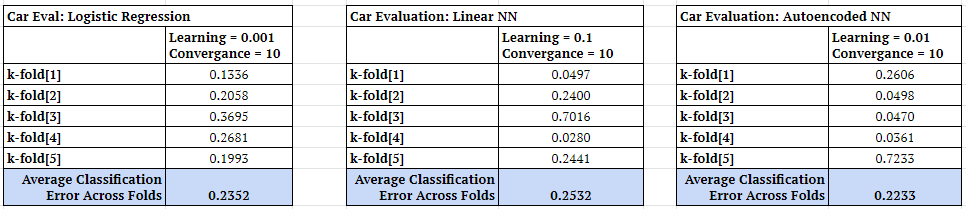
\includegraphics[scale=.7]{CarEval_All_Results}\newline
\end{table}

\begin{table}[h]
		\centering
		\caption{Breast Cancer: Linear Networks - Experimental Results}
		\label{tab:table2}
		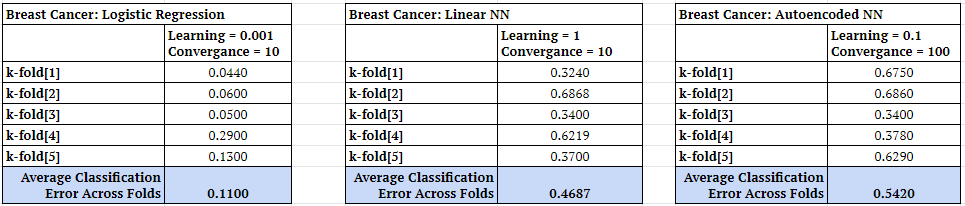
\includegraphics[scale=.7]{BC_All_Results}\newline
\end{table}

\begin{table}[h]
		\centering
		\caption{Congressional Vote: Linear Networks - Experimental Results}
		\label{tab:table3}
		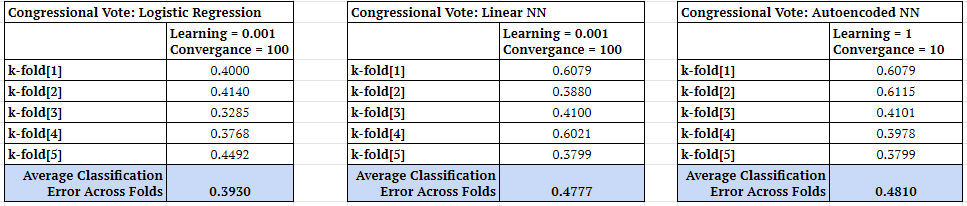
\includegraphics[scale=.7]{CongVote_All_Results}\newline
\end{table}
\newpage
\begin{table}[h]
	\centering
	\caption{Albalone: Linear Networks - Experimental Results}
	\label{tab:table4}
	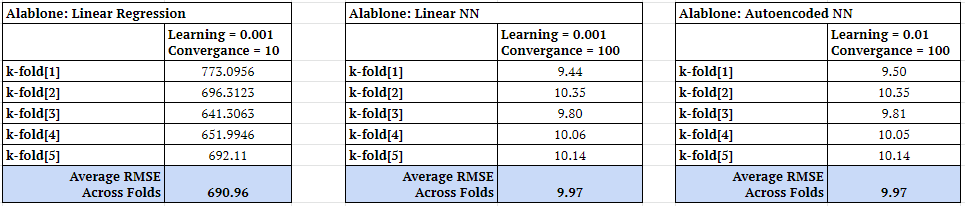
\includegraphics[scale=.7]{Albalone_All_Results}\newline
\end{table}

\begin{table}[h]
	\centering
	\caption{Computer Hardware: Linear Networks - Experimental Results}
	\label{tab:tale5}
	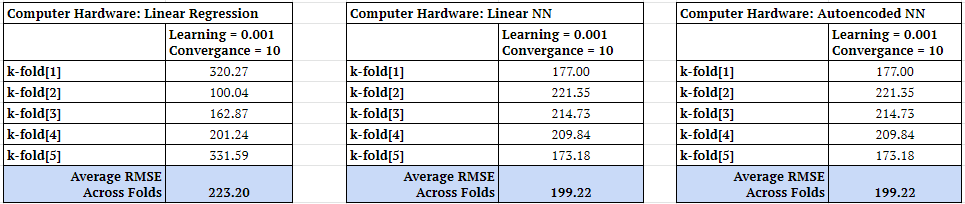
\includegraphics[scale=.7]{CompHW_All_Results}\newline
\end{table}

\begin{table}[h]
	\centering
	\caption{Forest Fires: Linear Networks - Experimental Results}
	\label{tab:table6}
	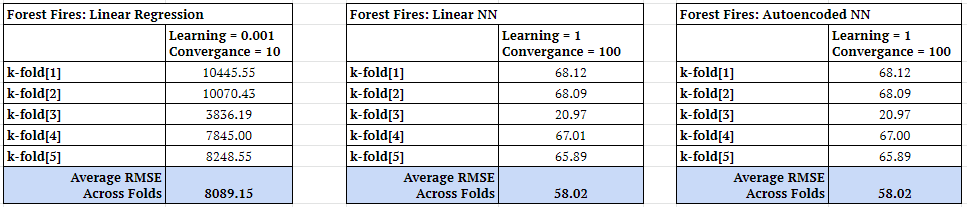
\includegraphics[scale=.7]{ForestFires_All_Results}\newline
\end{table}

\section{Discussion}
\hspace*{10mm} The hypothesis presented in this report was that the  Feed-Forward Network with an Auto Encoder will perform better than the Feed-Forward Back Propagation and Linear regression approaches on both the Classification and Regression problems.\\
\hspace*{10mm} Looking at the Classification data sets, it seemed that the Logisitc Regression performed best on average when compared with the Linear and Auto Encoded NN. Looking at the Regression data sets for the Linear NN and Auto Encoded NN, it seems that the Alabolne models were able to obtain a line of best fit as it had the smallest average RMSE across the folds.While the Computer Hardware had the largest average RMSE across the folds. A factor in this trend might be how the data has handled prior to being run through the algorithm. Some of the data in these data sets was categorical, so a One Hot encoding was applied. The Computer Hardware data set had the highest number of features that needed to be one hot encoded, when compared to Forest Fires (middle amount of one hot encoding) and Albalone (smallest amount of one hot encoding). This one hot encoding may have skewed the data in some way causing the RMSE to be highest for the Computer Hardware data set. For Regression data sets it was also noted that Auto Encoded NNs versus a regular Linear NN, seemed to have no impact on the RMSE that was obtained fold to fold. \\
\hspace*{10mm} One possible explanation for these results is that it was observed during the tuning process that very frequently the same fold error would be obtained fold to fold, this may indicate that in many cases the predictions being made by the algorithms were often tending to choose only one class label. This would mean that instead of learning a pattern the algorithm is just calculating the performance of the fold observations that were of that one class that it was predicting. This was noticed on the most on the computer hardware data set and as an area of future work should be examined to see if that truly is the root cause of the error. If that is the case, then it may be hard to make concise conclusions about the results of these modes.\\ 

\section{Conclusion}
\hspace*{10mm} Overall there seemed to be some trends that supported the general hypothesis. For regression data sets it seemed that the Linear NN would perform better than the Linear Regression. For classification the logistic regression performed best.\newline
\hspace*{10mm} A suggested area of future work, after fixing basic implementation details, would be to explore as part of the tuning process is the shape of the network. In the experiment the Neural Network that was built for the algorithm that included and input layer, 2 hidden layers and an output layer. This network could have been built with a different number of hidden layers and a variable number of nodes with in those hidden layers, that could have lead to different results. That structure of the network is an area that could be looked into for future work. \newline

\section{References}
1. Alpaydin, E. (2004). Introduction to machine learning (Oip). Mit Press. 

\newpage


\end{document}